\documentclass[10pt, twocolumn]{IEEEtran}
\usepackage[utf8]{inputenc}
\usepackage{graphicx}
\title{Granular synthesis for instrument makers}
\author{	
	\IEEEauthorblockN{Daniël Kamp\\}
    \IEEEauthorblockA{HKU University of the Arts Utrecht
    \\daniel.kamp@student.hku.nl}
    }
\date{April 2022}

\begin{document}

\maketitle

\begin{abstract}
This writing aims to provide insight into various forms of granular synthesis. It lists some existing implementations, explains the inner workings of such a system, and provides insight into human interfaces to use this technique.
\end{abstract}

\section*{Introduction}
This is where I write the introduction.

\section{What is granular synthesis?}
This section provides a brief history of granular synthesis, explains the parts that make up a system implementing this technique, and lists some popular and influential instruments.

\subsection{A brief history}
Granular synthesis as it's known today is a form of digital sound synthesis, which is based on the processing of small slices of sampled audio known as "grains". The underlying view on sound perception was first proposed by British physicist Dennis Gabor in an article titled "Acoustical Quanta and the Theory of Hearing", published in 1947. In this writing, Gabor theorized

\subsection{General system overview}
This section describes the general anatomy of a granular synthesizer, and gives a broad overview of the building blocks that make up such a system. It's expected that the reader has a basic knowledge of the workings of digital audio, and is familiar with the concept of sampling.

\begin{figure}[h!]
	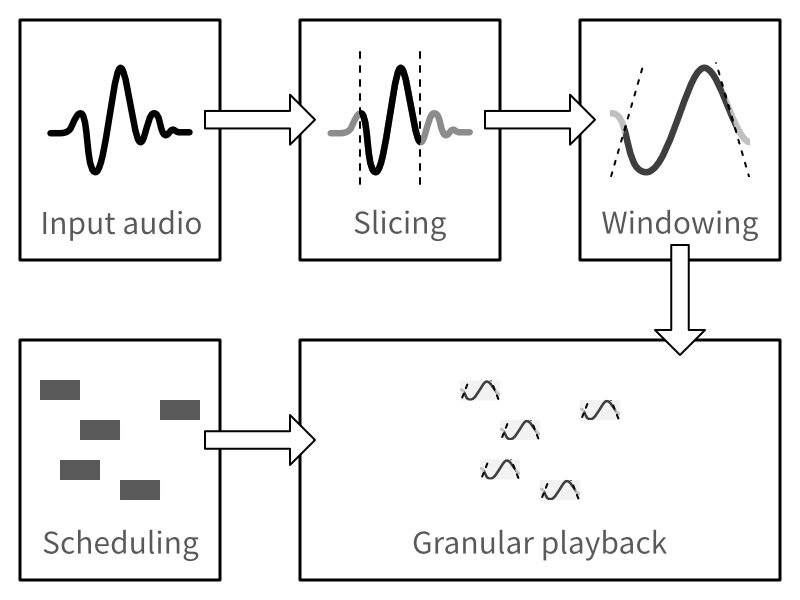
\includegraphics[width=\linewidth]{GranularDiagram.png}
	\caption{A simplified overview of a granular synthesis system.}
	\label{fig:block_diagram}
\end{figure}

\subsubsection{Sound source}
Here I write about samples, chopping, et cetera.
\subsubsection{Slicing}
Here I write about slicing (transients etc)
\subsubsection{Windowing and envelope}
Here I write about windowing, talk about some problems, and provide different envelope shapes and formulas.
\subsubsection{Various parameters}
Here I list various parameters that might be implemented along a granular system.
\begin{itemize}
\item{Stereo panning}
\item{Spread}
\item{something}
\end{itemize}

\subsection{Existing instruments}
This section lists a few instruments and effects that use granular synthesis. Author's note: I selected open-source instruments of which the source code is freely available to the public. This way, I can give an in-depth comparison of the inner workings of these instruments.

\subsubsection{Mutable Instruments' Clouds}
Clouds is a Eurorack module developed and produced by Émilie Gilet (Mutable Instruments). Both the hardware files (schematics, CAD-files) and firmware source code are open-source and publicly available.
What?
- Eurorack module
- Open-source hardware and firmware
- Granular effect with built-in sound source
How?
- Clouds triggers one grain at a time
- Clouds uses a predetermined amount of grains (64 max)
- Clouds uses Look Up Tables for almost everything (filter, windowing, etc)

\subsubsection{Tasty Chips GR-1}
Here I describe GR-1.

\subsubsection{Argotlunar}
Argotlunar is a realtime granular VST/AudioUnit plugin created by Michael Ourednik. The source code of this software is open source and available via Github.


\section{How does granular synthesis work?}
In this section I dive deeper into the inner workings of a granular system. I'll provide a schematic overview of some common implementations, and explain them further.

\subsection{Implementations}
This subsection lists different implementations.
\subsubsection{Sound sourcing and selection}
This part lists different methods of sound sourcing and sample selection:
- Microphone or audio input
- Sample-based granular synthesis
For sample selection:
- Randomized selection
- Transient selection
\subsubsection{Trigger algorithms}
Here I write about different trigger algorithms: when does a grain get triggered, what conditions exist, and how can this be controlled in a musical manner?
\subsubsection{Windowing algorithms and approaches}
Here I write about different approaches to windowing: look-up tables, real-time calculation, pre-calculation, etc.
Note: Mutable Instruments uses LUTs, I want to use runtime calculation (insert tested efficiency of both)

\subsection{Efficiency}
This subsection looks at variables that impact system performance, and how manufacturers handle those.

\section{How is granular synthesis used?}
This section looks at the human aspect of granular synthesis: what sounds does it produce, how is it controlled, and how can one play an instrument that uses this technique. KEEP THIS PART SHORT

\subsection{Human control}
This subsection looks at ways a human being can control a granular instrument. Common input methods like touch interfaces, sliders, knobs, and digital UIs are described and compared.

\subsection{Playability}
This subsection looks at how such instruments can be controlled in an artistic manner. It provides an insight into live performance methods and some useful macros (maybe).

\section*{Conclusions}
This section summarizes my findings from the research, and gives a careful recommendation on implementing such system based on these results.

\end{document}